% !TEX root = main.tex
In this section, we extend our approach to the setting where the =cost distributions $\{\set{F}_k\}_{k \in \set{K}}$ are initially unknown and the algorithm's classification, admission, and scheduling decisions should account for the need to learn these parameters online.

We first restrict our attention to \textsc{BACID}
admission rule: defer a job of type $k$ to human review if and only if $\beta \ell_k \geq Q_k(t)$ where $\ell_k = \min(\ell_k^+,\ell_k^-)$. When the cost distributions $\{\set{F}_k\}_{k \in \set{K}}$ are unknown, we cannot directly compute $\ell_k$ and we need to instead use some estimate for $\ell_k$. A canonical way to resolve this problem in, e.g., bandits with knapsacks \citep{agrawal2019bandits} is to use an optimistic estimate $\bar{\ell}_k(t)$. In particular, recall that $\set{D}(t)$ is the dataset collected in the first $t-1$ period. For each type~$k$, we can compute the sample-average estimation of $\ell_k^{+}$ and $\ell_k^{-}$ by $\hat{\ell}_k^+(t)=\frac{\sum_{(j,C_j)\in \set{D}(t) \colon \kappa(j) = k} C^+_j}{n_k(t)}$ and $\hat{\ell}_k^-(t)=\frac{\sum_{(j,C_j)\in \set{D}(t) \colon \kappa(j) = k} (C^-_j)}{n_k(t)}$ where  $n_k(t) = \sum_{(j,C_j) \in \set{D}(t)} \indic{\kappa(j)=k}$ is the number of samples from type $k$; if $n_k(t)=0$, we set $\hat{\ell}_k^+(t)=\hat{\ell}_k^-(t) = 0$. The sample-average of the mean cost $c_k$ is given by $\hat{c}_k(t) = \hat{\ell}_k^+(t) - \hat{\ell}_k^-(t)$. We can then compute a confidence bound of $c_k$ and an upper confidence bound of $\ell_k$ by
\begin{equation}\label{eq:conf-h}
\ubar{c}_k(t) = \max\left(-c_{\max},\hat{c}_k(t) - \sigma_{\max}\sqrt{\frac{8\ln t}{n_k(t)}}\right),~\bar{c}_k(t) = \min\left(c_{\max},\hat{c}_k(t) + \sigma_{\max}\sqrt{\frac{8\ln t}{n_k(t)}}\right)
\end{equation}
\begin{equation}\label{eq:conf-r}
\bar{\ell}_k(t) = \min\left(c_{\max},\min\left(\hat{\ell}_k^+(t), \hat{\ell}_k^-(t)\right) + 4\sigma_{\max}\sqrt{\frac{\ln t}{n_k(t)}}\right)
\end{equation}
where we recall that $\sigma_{\max}^2$ is the known variance proxy of cost $C_t$ and $c_{\max} \geq 1$ is a known upper bound on $\expectsub{k}{|C_t|}$ for any $t$, thus an upper bound on $|c_k|,\ell_k^{+}, \ell_k^{-},$ and $\ell_k$. We can then admit a job if and only if $\beta \bar{\ell}_k(t) \geq Q_k(t)$ (for type $\perp$, we set $\bar{\ell}_{\perp}(t) \equiv 0$). 

\subsection{Why Optimism-Only is Insufficient for Classification}\label{sec:opti-fail}
This optimistic admission rule gives a natural adaptation of \textsc{BACID} which we term \textsc{BACID.UCB}: 
\begin{enumerate}
\vspace{-\topsep}
\item reject job $t$ if and only if $\hat{c}_{\kappa(t)}(t) > 0$ (similar to Line~\ref{line:bacid-classify} in Algorithm~\ref{algo:bacid}); 
\vspace{-\topsep}
\item admit job $t$ if $\beta \bar{\ell}_{\kappa(t)}(t) \geq Q_{\kappa(t)}(t)$ (similar to Line~\ref{line:bacid-admit} in Algorithm~\ref{algo:bacid}); 
\vspace{-\topsep}
\item and schedule a type-$k$ job where $k$ maximizes $\mu_{k}Q_{k}(t)$ (same as Line~\ref{line:bacid-schedule} in Algorithm~\ref{algo:bacid}).\vspace{-\topsep}
\end{enumerate}
Such optimism-only heuristics generally work well in a constrained setting, such as bandits with knapsacks. The intuition is that assuming a valid upper confidence bound, we always admit a job that would have been admitted by $\textsc{BACID}$ with known cost distributions $\{\set{F}_k\}_{k \in \set{K}}$. If we admit a job that would not have been admitted by $\textsc{BACID}$, we obtain one more sample; this shrinks the confidence interval which, in turn, limits the number of mistakes and leads to efficient learning. 

Interestingly, this intuition does not carry over to our setting due to the additional error in downstream classification decisions of jobs that are not admitted, for which the sign of $\hat{c}_k(t)$ may differ from that of $c_k$. To illustrate this point, consider the following instance with $K=2$ types of jobs: texts (type-$1$) and videos (type-$2$). A text job has equal probability to have cost $\pm 1$ while a video job has cost equal to $0.01$ with probability $0.95$ and cost equal to $-0.01$ with probability $0.05$. Videos have a smaller absolute cost than texts and appear in the platform only after sufficient text jobs are in the review system; see Figure~\ref{fig:ucb-fail} for the exact instance parameters.

Proposition~\ref{prop:fail-to-learn} shows that \textsc{BACID.UCB} with initial knowledge of $\set{F}_1$ and knowledge that $|C_t| = 0.01$ conditioning on $\kappa(t) = 2$ does not review video jobs (for which $\set{F}_2$ is unknown) with high probability. Therefore, there is no video job in the dataset for the entire horizon, although there are $\Omega(T)$ arrivals of them. The proof, given in Appendix~\ref{app:prop-fail-to-learn}, relies on the fact that the queue of text jobs is always longer than that of video jobs and thus no video job will be scheduled for human review. As a result, when classifying video jobs, since there is no data, the algorithm estimates $\hat{c}_2(t) = 0$, and accepts all videos even if they are likely harmful, incurring $\Omega(T)$ regret.\footnote{We assume accepting a job when $\hat{c}_k(t) = 0$. If the algorithm rejects the job, the same issue exists by setting the cost distribution such that a video job has negative cost with probability $0.95$ and positive cost with probability $0.05$.}  

\begin{proposition}\label{prop:fail-to-learn}
There exists a setting such that for any $\beta > 100$ and $T \in (\beta / 2,\exp(\beta / 1152)]$, with probability at least $1 - 2/T$, there is no video job in the dataset $\set{D}(T+1)$ under $\textsc{BACID.UCB}$.
\end{proposition} 
\begin{figure}[!h]
  \centering
  \scalebox{0.75}{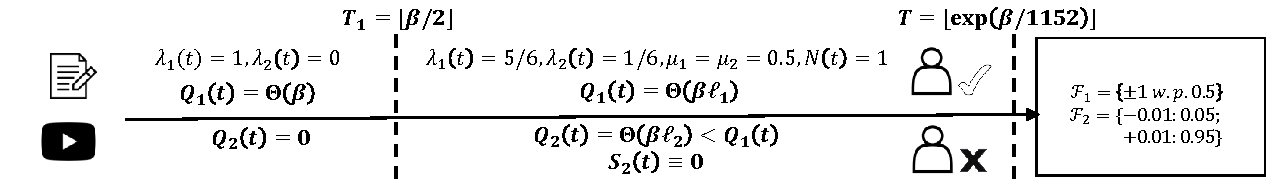
\includegraphics{figures/ucb_example.pdf}}
  \caption{An example where \textsc{BACID.UCB} fails to correctly classify video (type-$2$) jobs. Humans never review a video because the corresponding queue length is much smaller than that of texts.}
  \label{fig:ucb-fail} 
\end{figure}
\textsc{BACID.UCB} incurs linear regret in the above example as its decisions are inherently myopic to current rounds and disregard the importance of labels towards classification decisions in future rounds. Broadly speaking, optimism-only heuristics focus on the most optimistic estimate on the contribution of each action (in our setting, the admission decision) subject to a confidence interval and then select the action that maximizes this optimistic contribution in the current round. In our example, if we can only admit one type, the text jobs have larger idiosyncrasy loss due to their costs and thus the benefit of admitting a text job outweighs even the most optimistic estimate on the idiosyncrasy loss of video jobs in the current round. This mimics the admission rule of \textsc{BACID} which operates with known parameters and would never review a video job. Although always prioritizing text jobs is myopically beneficial in the current round, this means that we collect no new video data, thus harming our classification performance in the long run.

Though our proof of Proposition~\ref{prop:fail-to-learn} concerns the specific form of $\textsc{BACID.UCB}$, in Appendix~\ref{app:sim-fail-to-learn} we simulate several variants to $\textsc{BACID.UCB}$ in a setting similar to Figure~\ref{fig:ucb-fail}. The considered variants  include one with optimism in scheduling, one with discounted samples, and one with an initial exploration phase. We observe that the first two variants fail to collect enough samples of one type of jobs to ensure correct AI classification (similar to what happen for the video jobs in Figure~\ref{fig:ucb-fail}). Although initial exploration eases this issue, the third variant  leads to much higher loss and is not amenable to a setting with non-stationary arrivals. Our results thus highlight the robustness of the observation in Proposition~\ref{prop:fail-to-learn} that an optimism-only approach is insufficient for classification.

\subsection{Label-Driven Admission and Forced Scheduling for Classification}
The inefficiency of \textsc{BACID.UCB} suggests the need to complement the myopic nature of optimism-only approaches by a forward-looking exploration that enhances classification decisions. Our algorithm, \textsc{Optimistic and Label-driven Admission for Balanced Classification, Idiosyncrasy and Delay} or $\bacidol$ in short (Algorithm~\ref{algo:bacidol}) incorporates this forward-looking exploration and evades the shortcomings of optimism-only approaches. When a new job $t$ arrives, the platform rejects it if and only if the empirical average cost $\hat{c}_{\kappa(t)}(t)$ is positive. Unlike $\textsc{BACID}$ which assumes knowledge of $c_{\kappa(t)}$, when $\ubar{c}_{\kappa(t)}(t) < 0 < \bar{c}_{\kappa(t)}(t)$, we cannot confidently infer the sign of $c_{\kappa(t)}$ from the sign of $\hat{c}_{\kappa(t)}(t)$. 

To enhance future classification decisions on those jobs, we complement the optimism-based admission (Line~\ref{line:bacidol-admit}) with \emph{label-driven admission} (Line~\ref{line:bacidol-lda}). Specifically, we maintain a new \emph{label-driven queue} $\set{Q}^{\textsc{ld}}(t)$ and add the job to that queue ($E(t) = 1$) if (i) the queue is empty and (ii) there is high uncertainty on the sign of $\hat{c}_{\kappa(t)}(t)$, i.e., $\ubar{c}_{\kappa(t)}(t) \leq -\gamma$ and $\gamma \leq \bar{c}_{\kappa(t)}(t)$. For (i), we require the label-driven queue to be empty to avoid over-admission and to control its length over the horizon. For (ii), the parameter $\gamma$ avoids wasting reviewing capacity on \emph{indifferent} jobs,  for whom the difference in misclassification loss between acceptance and rejection is small (at most $\gamma$). If the job is admitted by the optimism-based admission ($E(t) = 0$, $\beta\bar{\ell}_{\kappa(t)}(t) \geq Q_{\kappa(t)}(t)$), we denote $A(t) = 1$. We stress that $Q_{\kappa(t)}(t)$ includes only jobs in the review queue $\set{Q}(t)$ and not in $\set{Q}^{\ld}(t)$. 

We use \emph{forced scheduling} to prioritize reviews for the label-driven queue. If $\set{Q}^{\ld}(t)$ is not empty, we review a job from $\set{Q}^{\ld}(t)$. Otherwise, we follow the \textsc{MaxWeight} scheduling (as in \textsc{BACID}): select a type $k$ that maximizes $\mu_{k}Q_{k}(t)$ and review the earliest waiting job in the review queue $\set{Q}(t)$ that has type $k$. We let $\psi_{k}(t) = 1$ if a type-$k$ job in $\set{Q}(t)$ is scheduled to review in period~$t$. 

\begin{algorithm}[H]
\LinesNumbered
\DontPrintSemicolon
  \caption{
  \textsc{Optimistic and Label-driven $\bacid$ ($\bacidol$)}}\label{algo:bacidol}
  \KwData{$T, \{\mu_k\}_{k \in \set{K}}, \sigma_{\max}, c_{\max}$} 
  \textbf{Admission parameters:} 
  $\beta = \sqrt{T / K}, \gamma = (T/(K\ln T))^{-1/3}$
  
  \For{$t = 1$ \KwTo $T$}{
    Observe a new job of type $\kappa(t)$ \\
    \lIf{$\hat{c}_{\kappa(t)}(t) > 0$}{$Y(t) \gets -1$ 
     \textbf{else} {$Y(t) \gets 1$}
    \tcp*[f]{Empirical Classification} \label{line:bacidol-classify}}
    \tcc{Label-Driven and Optimistic Admission}
Calculate $\ubar{c}_{\kappa(t)}(t),\bar{c}_{\kappa(t)}(t),\bar{\ell}_{\kappa(t)}(t)$ by \eqref{eq:conf-h} and \eqref{eq:conf-r} \label{line:bacidol-esti}\;
  \lIf{$\ubar{c}_{\kappa(t)}(t) < -\gamma < \gamma < \bar{c}_{\kappa(t)}(t)$ \emph{\textbf{and}} $|\set{Q}^{\ld}(t)|=0$}{
  $E(t) \gets 1$~\textbf{else} $E(t)=0$\label{line:bacidol-lda}}
    
    \lIf{$E(t) = 0$ \emph{\textbf{and}} $\beta \cdot \bar{\ell}_{\kappa(t)}(t) \geq Q_{\kappa(t)}(t)$}{
      $A(t) = 1$ \textbf{else} {$A(t) = 0$} 
    \label{line:bacidol-admit}
    }
\tcc{Forced Scheduling and \textsc{MaxWeight} Scheduling}
    
    \lIf{$\set{Q}^{\ld}(t) \neq \emptyset$}{$M(t)\gets$ the job in $\set{Q}^{\ld}(t)$} \label{line:bacidol-prio}
    \lElse{
    $k \gets \arg\max_{k' \in \mathcal{K}} \mu_{k'} \cdot Q_{k'}(t)$,~$M(t) \gets \text{first job in } \set{Q}_{k}(t) \text{ if any}$
    }
    \lIf{\emph{the review finishes (with probability $N(t) \cdot \mu_{\kappa(M(t))}$)}}
    {
      $\mathcal{S}(t) = M(t)$ \textbf{else} 
      $\mathcal{S}(t) = \perp$ 
    }
  }
\end{algorithm}
Our main result (Theorem~\ref{thm:bacidol}) is that, setting $\beta = \sqrt{T / K}, \gamma = (T/(K\ln T))^{-1/3}$, $\bacidol$ achieves a regret of $\tilde{O}(\sqrt{T})$ when there is a large margin $\eta\coloneqq \min(1,\min_{k \in \set{K}} |c_k|)$ and the number of types $K$ is small. In particular, the guarantee matches the lower bound $\Omega(\sqrt{T})$ in its dependence on $T$.  Even if there is no margin (so classification is difficult), $\bacidol$ still obtains a regret of $\tilde{O}(T^{2/3})$; this worse dependence is due to the classification difficulty and is unavoidable (Theorem~\ref{thm:bacidol-lowerbound}). 

\begin{theorem}\label{thm:bacidol}
The regret of $\bacidol$ is upper bounded by 
\[\reg^{\bacidol}(T) \lesssim 
K\sqrt{T\ln T} + \min\left(K\ln T / \eta^2, T^{2/3}(K\ln T)^{1/3}\right).\]
\end{theorem}
The below theorem shows that the worst-case $\tilde{O}(T^{2/3})$ regret is tight. The proof of this theorem is similar to standard arguments from multi-armed bandits and is deferred to Appendix~\ref{app:thm-bacidol-lowerbound}. 
\begin{theorem}\label{thm:bacidol-lowerbound}
When cost distributions are unknown, for any $T \geq 8$, there exists a setting such that $\reg^{\pi}(T)  \geq \frac{T^{2/3}}{36}$ for any feasible policy $\pi$.
\end{theorem}

Our proof of Theorem~\ref{thm:bacidol} relies on a loss decomposition of $\loss^{\bacidol}(T)$ that is similar to \eqref{eq:loss-decompose} 
but also captures the possible incorrect classification decisions. The incurred loss per period is $\left(Y(t)^+ \ell_k^{+}\right) + \left(Y(t)^-  \ell_k^{-}\right)$ instead of $\ell_k = \min(\ell_k^{+},\ell_k^{-})$ (recall that $Y(t) = 1$ means acceptance of the job and $Y(t) = -1$ means rejection of the job). 

Given that $\ell_k^{+}, \ell_k^{-} \leq c_{\max}$, we can upper bound $\expect{\loss^{\bacidol}(T)}$ by 
\begin{align}
&\hspace{0.1in}\underbrace{\expect{\sum_{t=1}^T \left(Y(t)^+(\ell_{\kappa(t)}^{+} - \ell_{\kappa(t)}) + Y(t)^-(\ell_{\kappa(t)}^{-}-\ell_{\kappa(t)})\right)(1 - A(t) - E(t))}}_{\text{Classification Loss}} \nonumber\\
&+  \underbrace{\expect{\sum_{t=1}^T  \ell_{\kappa(t)}(1 - A(t) - E(t))}}_{\text{Idiosyncrasy Loss}} +\underbrace{c_{\max}\expect{\sum_{k \in \set{K}} Q_k(T+1) + \left|\set{Q}^{\ld}(T+1)\right|}}_{\text{Relaxed Delay Loss}}.\label{eq:learning-loss-decompose}
\end{align}
Comparing \eqref{eq:learning-loss-decompose} with \eqref{eq:loss-decompose}, there is a new term on classification loss, which captures the loss when the classification $Y(t)$ is incorrect. We adjust the other terms to capture label-driven admission. The last term is called \emph{relaxed} delay loss because we upper bound the $\ell_k$ term in \eqref{eq:loss-decompose} by $c_{\max}.$

To bound the losses, we define  the minimum per-period review rate as $\hat{\mu}_{\min} = \min_{t \in [T], k \in \set{K}} N(t)\mu_k$. We focus on $T \geq 3$ and $K \leq T$ (the bound in Theorem~\ref{thm:bacidol} becomes trivial if $K > T$). Our bounds (Lemmas~\ref{lem:bacidol-delay},~\ref{lem:bacidol-class} and \ref{lem:bacidol-idio}) hold for general $\beta, \gamma$, and are proven in \ref{sec:bacidol-class} and \ref{sec:bacidol-idio} respectively. The lemmas are defined for $T \geq 3$ and $K \leq T$. The proof of Theorem~\ref{thm:bacidol} (provided in Appendix \ref{app:thm-bacidol}) directly combines the lemmas.
\begin{lemma}\label{lem:bacidol-delay}
For any $\beta \geq 1 / c_{\max}$, the Relaxed Delay Loss of $\bacidol$ is at most $3c^2_{\max} K\beta .$
\end{lemma}
\begin{proof}
For the review queue $\set{Q}$, we admit a type-$k$ job into $\set{Q}$ only if $\beta \bar{\ell}_k(t)\leq Q_k(t)$ and $\bar{\ell}_k(t) \leq c_{\max}$. As in the proof of Lemma~\ref{lem:known-delay}, the queue length is bounded by $Q_k(t) \leq \beta c_{\max} + 1 \leq 2\beta c_{\max}$. Moreover, the label-driven queue has at most one job by our admission rule on Line~\ref{line:bacidol-lda} of Algorithm~\ref{algo:bacidol}. The relaxed delay loss is thus upper bounded by $c_{\max}K(2\beta c_{\max}) + 1 \leq 3c^2_{\max}K\beta.$
\end{proof}

\begin{lemma}\label{lem:bacidol-class}
For any $0 < \gamma \leq 1$, the Classification Loss of $\bacidol$ is at most 
\[
\gamma \indic{\gamma \geq \eta} T + \frac{38c_{\max}K\sigma^2_{\max}\ln T}{\max(\eta,\gamma)^2\hat{\mu}_{\min}} + 5Kc_{\max}.
\]
\end{lemma}
\begin{lemma}\label{lem:bacidol-idio}
For any $\beta \geq 1 / c_{\max}, \gamma \in (0,1]$, the Idiosyncrasy Loss of $\bacidol$ is at most
\[
\loss^\star(T) + \frac{T}{\beta}+\frac{76c_{\max}K\sigma^2_{\max}\ln T}{\max(\eta,\gamma)^2\hat{\mu}_{\min}}+20Kc_{\max}\left(\sqrt{T\ln T} + \beta c_{\max}\right).
\]
\end{lemma}

\subsection{Bounding the Classification Loss (Lemma~\ref{lem:bacidol-class})}\label{sec:bacidol-class}
A key ingredient in the proofs of Lemmas  \ref{lem:bacidol-class} and \ref{lem:bacidol-idio} is to provide an upper bound on the number of periods that the label-driven queue is non-empty. Given that $\set{Q}^{\ld}(t)$ has at most one job at any period $t$, letting $Q^{\ld}(t) = |\set{Q}^{\ld}(t)|$, this is equal to $\expect{\sum_{t=1}^T Q^{\ld}(t)}$. This quantity allows to bound 1) the number of jobs which we do not admit into the label-driven queue despite not being able to confidently estimate the sign of their expected cost and 2) the number of periods that we do not follow \textsc{MaxWeight} scheduling.

Our first lemma connects $\expect{\sum_{t=1}^T Q^{\ld}(t)}$ to the number of jobs admitted to the label-driven queue $\set{Q}^{\textsc{ld}}(t)$. The proof (Appendix~\ref{app:lem-connect-et-qe}) relies on two facts: (1) the queue $\set{Q}^{\textsc{ld}}(t)$ has length at most one; and (2) each job stays in the queue for at most $1 / \hat{\mu}_{\min}$ periods in expectation. 
\begin{lemma}\label{lem:connect-et-qe}
The total length of the label-driven queue is at most $\expect{\sum_{t=1}^T Q^{\ld}(t)} \leq \frac{\expect{\sum_{t=1}^TE(t)}}{\hat{\mu}_{\min}}$.
\end{lemma}
Our second lemma applies concentration bounds (Appendix~\ref{app:lem-prob-good-event}) to show that the event $\set{E}_{k,t} = \{c_k \in [\ubar{c}_k(t),\bar{c}_k(t)],\ell_k \leq \bar{\ell}_k(t)\}$ (confidence bounds are valid) holds with high probability. A challenge in establishing this lemma is to show that $C_t^+$ and $C_t^-$ are also sub-Gaussian given that $C_t$ is sub-Gaussian, which we establish with techniques from \cite{kontorovich2014concentration}.
\begin{lemma}\label{lem:prob-good-event}
For any $k,t$, the confidence bounds \eqref{eq:conf-h},\eqref{eq:conf-r} are valid with probability $\Pr\{\set{E}_{k,t}\} \geq 1 - 4t^{-3}$.
\end{lemma}

Our next lemma (proof in Appendix~\ref{app:lem-bound-sum-ek}) bounds $\expect{\sum_{t=1}^T E(t)}$ via considering the type-$k$ confidence interval when the last type-$k$ job is admitted to the label-driven queue $\set{Q}^{\textsc{ld}}$.
\begin{lemma}\label{lem:bound-sum-ek}
The label-driven queue admits at most
$\expect{\sum_{t=1}^T E(t)} \leq \frac{38K\sigma^2_{\max}\ln T}{\max(\eta,\gamma)^2}$ jobs.
\end{lemma}

To show Lemma~\ref{lem:bacidol-class} we also need the below lemma (proof in Appendix~\ref{app:lem-bacidol-class-err}), which establishes a bound on the type-$k$ period-$t$ classification loss \[Z_k(t) = \Lambda_k(t)\left(Y(t)^+(\ell_k^{+} - \ell_k) + Y(t)^-(\ell_k^{-}-\ell_k)\right)(1 - A(t) - E(t)).\]

\begin{lemma}\label{lem:bacidol-class-err}
For any type $k$ and period $t$,  $Z_k(t)\indic{\set{E}_{k,t}} \leq \left(\gamma \indic{\gamma \geq \eta} + c_{\max}Q^{\ld}(t)\right)\Lambda_k(t).$
\end{lemma}
\begin{proof}[Proof of Lemma~\ref{lem:bacidol-class}]
By definition, the total classification loss is $\expect{\sum_{t=1}^T \sum_{k \in \set{K}} Z_k(t)}$. As a result,
\begin{align*}
\expect{\sum_{t=1}^T \sum_{k \in \set{K}} Z_k(t)} &\leq \expect{\sum_{t=1}^T \sum_{k \in \set{K}} Z_k(t)\indic{\set{E}_{k,t}}} + c_{\max}\sum_{t=1}^T \sum_{k \in \set{K}} \Pr\{\set{E}_{k,t}^c\} \tag{$Z_k(t)\leq c_{\max}$}\\
&\leq \expect{\sum_{t=1}^T \sum_{k \in \set{K}} Z_k(t)\indic{\set{E}_{k,t}}} + Kc_{\max}\sum_{t=1}^T \frac{4}{t^3} \tag{By Lemma~\ref{lem:prob-good-event}}\\
&\leq \expect{\sum_{t=1}^T \left(\gamma \indic{\gamma \geq \eta} + c_{\max}Q^{\ld}(t)\right)} + 5Kc_{\max}\tag{By Lemma~\ref{lem:bacidol-class-err}} \\
&\hspace{-0.5in}\leq \gamma \indic{\gamma \geq \eta} T + \frac{38c_{\max}K\sigma^2_{\max}\ln T}{\max(\eta,\gamma)^2\hat{\mu}_{\min}} + 5Kc_{\max}.\tag{By Lemmas~\ref{lem:connect-et-qe},~\ref{lem:bound-sum-ek}}
\end{align*}
\end{proof}

\subsection{Bounding 
the Idiosyncrasy Loss (Lemma~\ref{lem:bacidol-idio})}\label{sec:bacidol-idio}
We follow a similar strategy as in the proof of Lemma~\ref{lem:known-idiosyncrasy}, but we encounter three new challenges due to the algorithmic differences between \textsc{BACID} and $\bacidol$. 

Our first challenge arises because of the additional label-driven admission. Without the label-driven admission, we would admit a type-$k$ job to the review queue $\set{Q}(t)$ in period $t$ if its (optimistic) idiosyncrasy loss outweighs the delay loss, i.e., $\bar{A}_k(t) = \Lambda_k(t)\indic{\beta \bar{\ell}_k(t) \geq Q_k(t)}$ is equal to one. However, we now only admit such a job to $\set{Q}(t)$ if it is not admitted to the label-driven queue $\set{Q}^{\ld}(t)$, i.e., the real admission decision is $A_k(t) = \bar{A}_k(t)(1-E(t))$. The following Lyapunov function defined based on only the length of $\set{Q}(t)$ accounts for this difference and offers an analogue of Lemma \ref{lem:connect-idio-lag}, which we prove in Appendix~\ref{app:lem-bacidol-idio-lag}. 
\[
L(t) = \beta\sum_{t'=1}^{t-1}\ell_{\kappa(t')}(1-A(t') - E(t'))+\frac{1}{2}\sum_{k \in \set{K}}Q_k^2(t).
\]
\begin{lemma}\label{lem:bacidol-idio-lag}
The expected Lagrangian of $\bacidol$ upper bounds the idiosyncrasy loss by:
\[
\beta\expect{\sum_{t=1}^T \ell_{\kappa(t)}(1 - A(t) - E(t))} \leq \expect{L(T+1) - L(1)} \leq T + \sum_{t=1}^T \expect{f_t(\bolds{\bar{A}}(t),\bolds{\psi}(t),\bolds{Q}(t))}.
\]
\end{lemma}
We next bound the right hand side of Lemma~\ref{lem:bacidol-idio-lag}. By Lemma~\ref{lem:lagrang-bacid}, we know how to bound this quantity when admission and scheduling decisions are made according to \textsc{BACID}, i.e., $A_k^{\bacid}(t) = \indic{\beta \ell_k \geq Q_k(t)}\Lambda_k(t)$ and $\psi_k^{\bacid}(t) = \indic{k = \arg\max_{k' \in \set{K}} \mu_{k'} Q_{k'}(t)}$. To bound the Lagrangian under $\bacidol$, we connect it to its analogue under $\bacid$ via the \emph{regret in Lagrangian}:
\begin{align*}
\textsc{RegL}(T) &=\expect{\sum_{t=1}^T f_t(\bolds{\bar{A}}(t), \bolds{\psi}(t), \bolds{Q}(t)) - f_t(\bolds{A}^{\bacid}(t), \bolds{\psi}^{\bacid}(t), \bolds{Q}(t))} \\
&\hspace{-0.5in}= \underbrace{\expect{\sum_{t=1}^T \sum_{k\in\set{K}} (A_k^{\bacid}(t) - \bar{A}_k(t))(\beta \ell_k-Q_k(t))}}_{\textsc{RegA}(T)} + \underbrace{\expect{\sum_{t=1}^T \sum_{k \in \set{K}} (\psi_k^{\bacid}(t) - \psi_k(t))Q_k(t)\mu_k N(t)}}_{\textsc{RegS}(T)}.
\end{align*}
Our second challenge is to upper bound the regret in admission $\textsc{RegA}(T)$. This regret arises because, unlike $\bacid$ which admits based on the ground-truth per-period idiosyncrasy loss $\ell_k$, $\bacidol$ uses the optimistic estimation $\bar{\ell}_k(t)$. Different from works in bandits with knapsacks, to upper bound this regret, the following lemma also needs to account for the endogenous queueing delay in label acquisition. The proof in Appendix~\ref{app:lem-bacidol-rega} addresses this challenge by connecting the number of unobserved labels with the queue length of the system and using the fact that the queue length is always bounded under our admission decisions. 

\begin{lemma}\label{lem:bacidol-rega}
The regret in admission is $\textsc{RegA}(T) \leq 20K\beta^2c^2_{\max}+16K\beta c_{\max}\sqrt{T\ln T}. $
\end{lemma}
Our third challenge is to bound the regret in scheduling $\textsc{RegS}(T)$. Unlike $\bacid$ which schedules based on \textsc{MaxWeight}, $\bacidol$ prioritizes jobs in the $\set{Q}^{\ld}(t)$. The effect of those deviations is bounded in the next lemma (proof in Appendix~\ref{app:lem-bacidol-regs}), using Lemmas \ref{lem:connect-et-qe} and \ref{lem:bound-sum-ek}.
\begin{lemma}\label{lem:bacidol-regs}
The regret in scheduling is  $\textsc{RegS}(T) \leq \frac{76\beta c_{\max}K\sigma^2_{\max}\ln T}{\max(\eta,\gamma)^2\hat{\mu}_{\min}}$.
\end{lemma}
\begin{proof}[Proof of Lemma~\ref{lem:bacidol-idio}]
By Lemma~\ref{lem:bacidol-idio-lag}, the idiosyncrasy loss is upper bounded by
\begin{align*}
\beta\expect{\sum_{t=1}^T \ell_{\kappa(t)}(1 - A(t) - E(t))} &\leq T + \sum_{t=1}^T \expect{f_t(\bolds{\bar{A}}(t), \bolds{\psi}(t), \bolds{Q}(t))} \\
&= T + \sum_{t=1}^T \expect{f_t(\bolds{A}^{\bacid}(t), \bolds{\psi}^{\bacid}(t),\bolds{Q}(t))} + \textsc{RegL}(T)\\
&\leq T + \beta \loss^\star(T) + \textsc{RegA}(T) + \textsc{RegS}(T) \tag{By Lemma~\ref{lem:lagrang-bacid}} \\
&\hspace{-1in}\leq T + \beta \loss^\star(T)+ 20K\beta^2c^2_{\max} + 16K\beta c_{\max}\sqrt{T\ln T} + \frac{76\beta c_{\max}K\sigma^2_{\max}\ln T}{\max(\eta,\gamma)^2\hat{\mu}_{\min}} \tag{By Lemmas~\ref{lem:bacidol-rega} and \ref{lem:bacidol-regs}} \\
&\hspace{-1in}\leq T + \beta \loss^\star(T)+\frac{76\beta c_{\max}K\sigma^2_{\max}\ln T}{\max(\eta,\gamma)^2\hat{\mu}_{\min}}+20K\beta c_{\max}\left(\sqrt{T\ln T} + \beta c_{\max}\right).
\end{align*}
Dividing both sides of the inequality by $\beta$ gives the desired result.
\end{proof}